% Chapter 3 -- tests and experimental results.
\chapter{测试与结果}\label{ch:results}

\section{测试策略}

测试分为四层，覆盖“规格是否正确”和“实现是否忠实于规格”两个问题：

\begin{enumerate}
  \item \textbf{单元测试}：Catch2 v3（vendored，仅测试可执行文件链接），覆盖 tokenizer、stemmer、dict、index、query、stopwords、count、bptree；
  \item \textbf{黄金样例}：讲义中的四文档例子，逐项比对 posting 表；
  \item \textbf{独立对拍}：用 Python 独立实现同一规格，与 C++ 输出逐字节或逐项比较；
  \item \textbf{不变量与边界}：索引加载校验、损坏文件、空查询、停用词查询、未知词、B+Tree 与 \code{std::map} oracle 对拍等。
\end{enumerate}

\code{ctest} 注册了 8 个单元测试可执行文件，外加 \code{mse_stats} / \code{rfc_stats} 冒烟测试、v1/v2 的 brute-force 与磁盘词典对拍，以及 v1/v2 的短语级对拍，共 \textbf{18 项}（Python 可选；未安装时跳过）。

\section{单元测试结果}

本次在 WSL2 加 g++ 15.2（\code{-std=c++17 -O1}）下编译并运行八个测试可执行文件，全部通过（表~\ref{tab:unit-tests}）。

\begin{table}[H]
  \centering
  \caption{单元测试结果}
  \label{tab:unit-tests}
  \small
  \begin{tabularx}{\linewidth}{@{}l r r X@{}}
    \toprule
    测试文件 & TEST\_CASE 数 & 断言数 & 结果 \\
    \midrule
    \code{test_tokenizer} & 2 & 24 & 通过 \\
    \code{test_stemmer} & 7 & 101 & 通过 \\
    \code{test_dict} & 6 & 50 & 通过（新增 \code{std::map}） \\
    \code{test_index} & 8 & 248 & 通过（新增 v2/压缩链） \\
    \code{test_query} & 7 & 26 & 通过 \\
    \code{test_stopwords} & 3 & 11 & 通过 \\
    \code{test_count} & 3 & 47 & 通过（熵特征与派生规则） \\
    \code{test_bptree} & 10 & 84,648 & 通过（\code{std::map} oracle 加文件往返） \\
    \midrule
    合计 & 46 & 85,155 & 全部通过 \\
    \bottomrule
  \end{tabularx}
\end{table}

\code{test_bptree} 的 8.4 万条断言主要来自“对每个键与 \code{std::map} oracle 逐项比较”的三档页宽和对抗性键测试；断言数大不代表用例多，而是每个键的读、写、范围扫描都被显式核对。此外，\code{mse stats} 冒烟测试确认语料仍为 195 个文档；\code{crosscheck_brute_force} 对全词表对拍通过（见 3.4 节）。

\section{黄金样例：讲义四文档}

\code{tests/fixtures/golden4/} 复刻了讲义 1.2 节的四文档例子（表~\ref{tab:golden4-docs}）。

\begin{table}[H]
  \centering
  \caption{黄金样例的四篇文档}
  \label{tab:golden4-docs}
  \begin{tabularx}{\linewidth}{@{}r X@{}}
    \toprule
    docID & 文本 \\
    \midrule
    1 & Gold silver truck \\
    2 & Shipment of gold damaged in a fire \\
    3 & Delivery of silver arrived in a silver truck \\
    4 & Shipment of gold arrived in a truck \\
    \bottomrule
  \end{tabularx}
\end{table}

原始构建（无停用词、无词干化）得到 4 个文档、11 个词、25 个 token。逐项比对结果见表~\ref{tab:golden4-postings}。

\begin{table}[H]
  \centering
  \caption{黄金样例的 posting 表}
  \label{tab:golden4-postings}
  \begin{tabularx}{0.72\linewidth}{@{}l X@{}}
    \toprule
    词 & posting（docID, tf） \\
    \midrule
    a & (2,1) (3,1) (4,1) \\
    arrived & (3,1) (4,1) \\
    damaged & (2,1) \\
    delivery & (3,1) \\
    fire & (2,1) \\
    gold & (1,1) (2,1) (4,1) \\
    in & (2,1) (3,1) (4,1) \\
    of & (2,1) (3,1) (4,1) \\
    shipment & (2,1) (4,1) \\
    silver & (1,1) (3,2) \\
    truck & (1,1) (3,1) (4,1) \\
    \bottomrule
  \end{tabularx}
\end{table}

位置校验：doc1 中 \code{silver} 在 position 1；doc3 中 \code{silver} 在 positions 2 和 6。

\textbf{一处参考材料复核}：讲义表格把 \code{a} 记为 (2,1)(4,1)，但示例句子中 doc3 的原文是 “Delivery of silver arrived in \textbf{a} silver truck”，按句子重算应为 (2,1)(3,1)(4,1)。项目以句子为建索引的事实依据，测试中显式记录了这一差异。这一点也说明：引用示例时应以原始文本为准，而不是以二手表格为准。停用词版本（过滤 \code{a/of/in}）得到 8 个词；\code{silver} 在 doc3 中的位置重新编号为 1 和 3，验证了“停用词不占 position”的语义。

\section{独立对拍}

对拍的价值在于：如果 C++ 与 Python 两边都错，只有“同错”才会通过；因此规格中的每个模糊点都必须在两边独立写成一致的行为。本项目的对拍结果见表~\ref{tab:crosscheck}。

{\small
\begin{longtable}{@{}>{\raggedright\arraybackslash}p{0.40\linewidth}
                    >{\raggedright\arraybackslash}p{0.21\linewidth}
                    >{\raggedright\arraybackslash}p{0.33\linewidth}@{}}
  \caption{独立对拍结果}\label{tab:crosscheck} \\
  \toprule
  对拍项 & 规模 & 结果 \\
  \midrule
  \endfirsthead
  \toprule
  对拍项 & 规模 & 结果 \\
  \midrule
  \endhead
  \bottomrule
  \endlastfoot
  逐文档 token 数（C++ tokenizer vs Python） & 195 文档 & 100\% 一致，866,626 token \\
  \code{wordcount.csv} 默认配置 & 25,705 行 & 逐字节一致 \\
  \code{wordcount.csv --keep-speakers} & 25,705 行 & 逐字节一致 \\
  \code{wordcount.csv --stop-words} & 556,866 kept / 309,760 removed & 逐字节一致 \\
  \code{wordcount.csv --stem} & 14,947 词干 & 逐字节一致（NLTK \code{MARTIN_EXTENSIONS}） \\
  \code{wordcount.csv --stem --stop-words} & 14,937 词干 & 逐字节一致 \\
  词典层随机工作负载 & 20,000 次操作 / 300 词 & splay 与 hash 词表完全一致 \\
  索引文件（splay vs hash） & 3,685,655 B & 逐字节一致 \\
  索引文件（splay vs std::map） & 3,685,655 B & 逐字节一致 \\
  \code{brute_force.py} 全词表对拍（v1） & 14,937 词干 & df、tf、docID、positions 全项一致 \\
  \code{brute_force.py} 全词表对拍（v2 压缩） & 14,937 词干 & 独立解析 v2 文件，全项一致 \\
  \code{brute_force.py} raw 版 & 25,705 词 & 全项一致（见 notes.md 记录） \\
  块式构建 vs 内存构建 & 17 个 run / 4,166,556 B 临时 & 索引逐字节一致 \\
  磁盘 B+Tree \code{dump --verify-all} & 14,937 词 & 逐词 posting 与全量加载 0 差异 \\
  磁盘词典查询 vs 全量加载 & \code{osric} 单词查询 & 文本与 JSON 输出逐字节一致 \\
  短语查询 vs 独立扫描（v1） & 303 条随机短语 & 返回文档集 100\% 一致 \\
  短语查询 vs 独立扫描（v2） & 303 条随机短语 & 返回文档集 100\% 一致 \\
  RFC 语料（\code{data2/}）全链路 & 3 文档 / 2,660 词干 & count CSV 逐字节一致；brute-force 全项一致 \\
\end{longtable}
}

\code{brute_force.py} 是独立实现的第二套索引路径：它重新扫描 \code{data/text/}，用独立的 tokenizer、停用词表和 NLTK Porter 重建 posting，同时用独立的二进制解析器读取 \code{index.bin}，然后逐词比较。它不是“调用 C++ 的结果再比较”，而是真正从原始数据重建期望值。

\section{任务 (1) 结果：词频与停用词}

默认配置（只统计正文行）的统计结果：

\begin{lstlisting}[language=,basicstyle=\ttfamily\small]
documents: 195
tokens   : 866,626
distinct : 25,705
hapax    : 9,753 (tf = 1)
\end{lstlisting}

top 10 词项见表~\ref{tab:top10}。

\begin{table}[H]
  \centering
  \caption{词频 top 10}
  \label{tab:top10}
  \small
  \begin{tabularx}{\linewidth}{@{}r l r r r r@{}}
    \toprule
    rank & term & tf & df & df\_ratio & tf\_share \\
    \midrule
    1 & the & 28,436 & 177 & 90.8\% & 3.28\% \\
    2 & and & 25,553 & 189 & 96.9\% & 2.95\% \\
    3 & i & 21,131 & 154 & 79.0\% & 2.44\% \\
    4 & to & 20,302 & 187 & 95.9\% & 2.34\% \\
    5 & of & 16,976 & 175 & 89.7\% & 1.96\% \\
    6 & a & 14,527 & 138 & 70.8\% & 1.68\% \\
    7 & you & 13,998 & 75 & 38.5\% & 1.62\% \\
    8 & my & 12,934 & 159 & 81.5\% & 1.49\% \\
    9 & that & 11,513 & 172 & 88.2\% & 1.33\% \\
    10 & in & 11,479 & 181 & 92.8\% & 1.32\% \\
    \bottomrule
  \end{tabularx}
\end{table}

\begin{figure}[H]
  \centering
  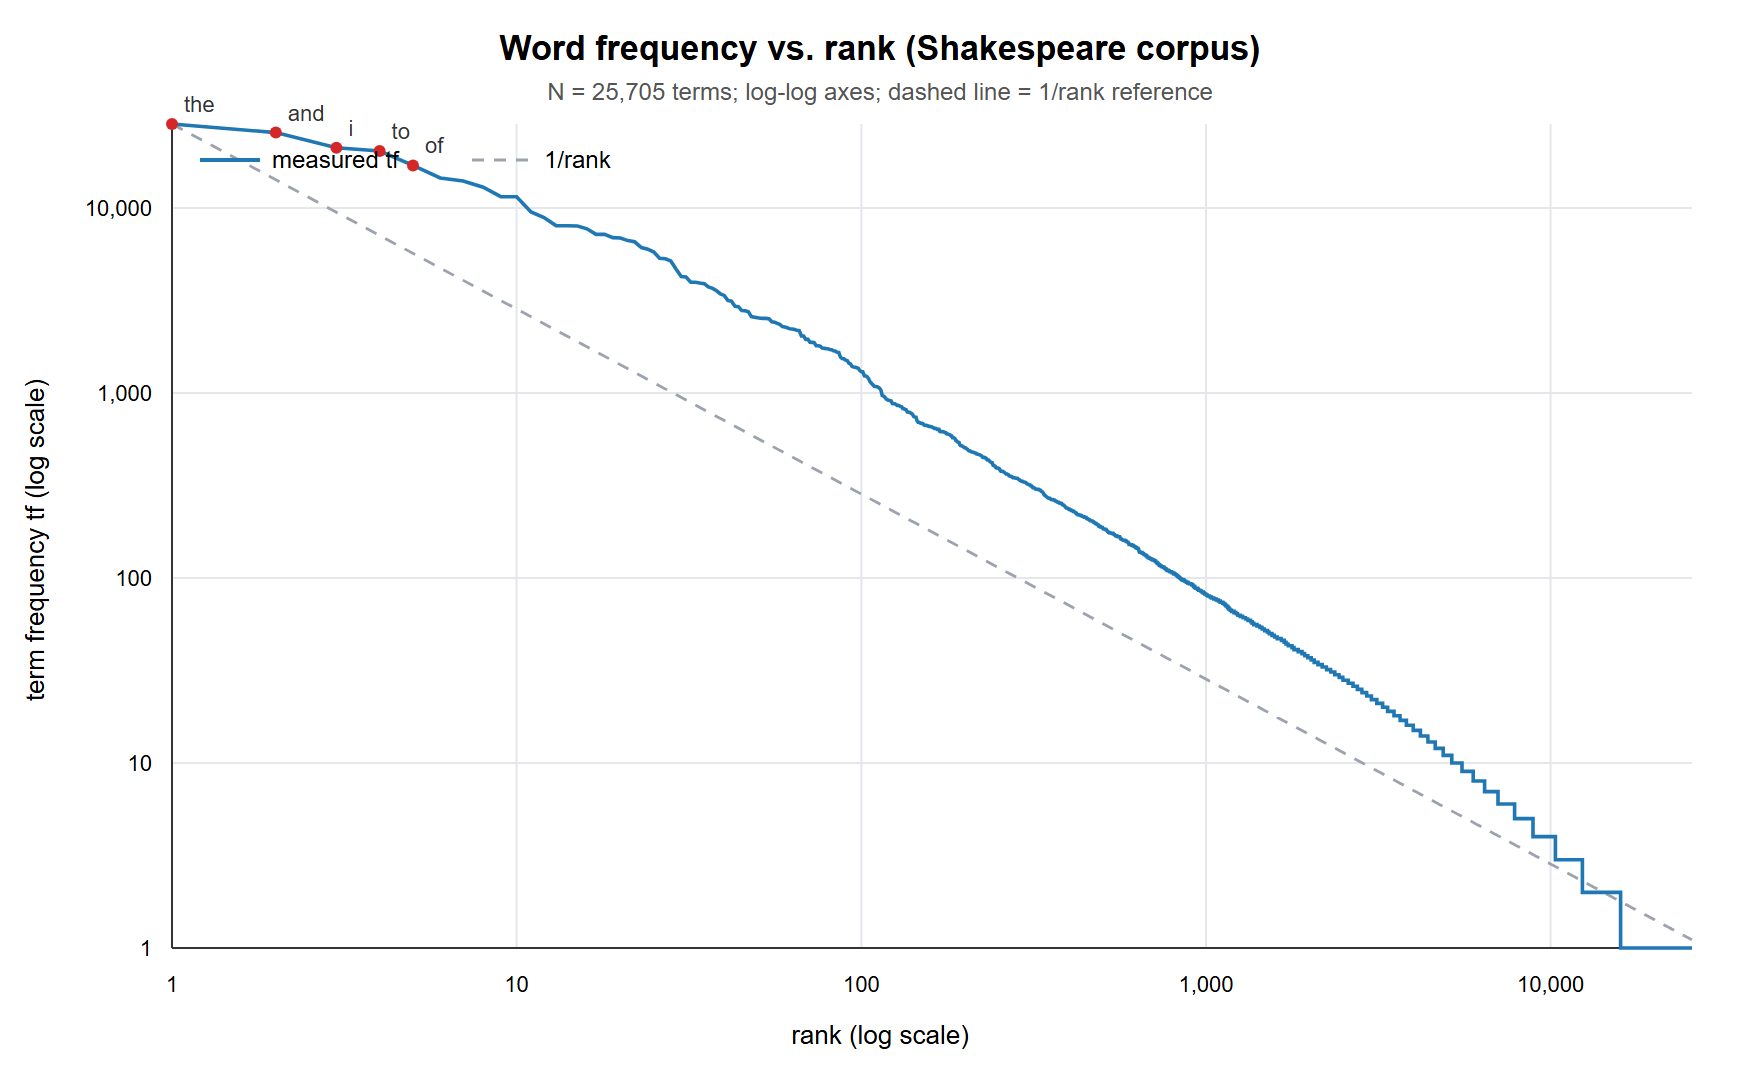
\includegraphics[width=0.92\linewidth]{figures/zipf.png}
  \caption{莎士比亚语料的 Zipf 分布。横轴为词频排名，纵轴为 tf；虚线为 1/rank 参考线。少量高频词占据大部分 token，长尾由大量 hapax 组成。}
  \label{fig:zipf}
\end{figure}

\code{stop_candidate} 粗筛（$df\_ratio \ge 0.75$ 且 $tf\_share \ge 0.1\%$）得到 9 个词：\code{the}、\code{and}、\code{i}、\code{to}、\code{of}、\code{my}、\code{that}、\code{in}、\code{but}。最终按 2.4.2 节的 0.40 候选带加人工结构判定得到 39 词停用表，覆盖 35.74\% 的 token。滤波前后对比见表~\ref{tab:filter-variants}。

\begin{table}[H]
  \centering
  \caption{词频统计的四种配置}
  \label{tab:filter-variants}
  \small
  \begin{tabularx}{\linewidth}{@{}l r r r X@{}}
    \toprule
    配置 & token 数 & distinct & hapax & 说明 \\
    \midrule
    不过滤 & 866,626 & 25,705 & 9,753 & 基线 \\
    \code{--stop-words} & 556,866 & 25,666 & 9,753 & removed 309,760（35.74\%） \\
    \code{--stem} & 866,626 & 14,947 & 4,843 & 词干化合并词形 \\
    \code{--stem --stop-words} & 556,866 & 14,937 & 4,846 & 正式索引配置 \\
    \bottomrule
  \end{tabularx}
\end{table}

\subsection{熵特征与自动停用词（Bonus）}

\code{mse count} 新增 \code{entropy}、\code{entropy_norm}、\code{entropy_rate_norm} 三列。代表性读数见表~\ref{tab:entropy-values}。

\begin{table}[H]
  \centering
  \caption{熵特征的代表性读数}
  \label{tab:entropy-values}
  \small
  \begin{tabularx}{\linewidth}{@{}l r r r r X@{}}
    \toprule
    词 & tf & df & entropy\_norm & entropy\_rate\_norm & 类型 \\
    \midrule
    the & 28,436 & 177 & 0.724 & 0.975 & 功能词 \\
    and & 25,553 & 189 & 0.721 & 0.979 & 功能词 \\
    it & 8,001 & 100 & 0.805 & 0.969 & 功能词 \\
    is & 9,508 & 137 & 0.760 & 0.972 & 功能词 \\
    love & 2,224 & 127 & 0.789 & 0.927 & 内容词 \\
    sweet & 852 & 87 & 0.838 & 0.893 & 内容词 \\
    king & 1,368 & 40 & 0.818 & 0.826 & 内容词 \\
    heart & 1,086 & 70 & 0.894 & 0.831 & 内容词 \\
    osric & 3 & 1 & 0 & 0 & 专名 \\
    \bottomrule
  \end{tabularx}
\end{table}

原始熵排序反直觉（\code{the} 0.724 小于 \code{man} 0.941），长度归一化后功能词与内容词才分开。\code{mse stopwords --derive --min-df-ratio 0.4 --min-entropy-rate 0.93} 自动得到 39 词，与人工表重叠 35；差异见 2.4.4 节。

三套索引（均使用 \code{--stem}）的对比见表~\ref{tab:three-indexes}。

\begin{table}[H]
  \centering
  \caption{三种停用词配置的索引规模}
  \label{tab:three-indexes}
  \small
  \begin{tabularx}{\linewidth}{@{}X r r r r@{}}
    \toprule
    停用词 & tokens & terms & postings & 索引字节 \\
    \midrule
    无 & 866,626 & 14,947 & 121,903 & 4,958,598 \\
    静态 39（\code{data/stopwords.txt}） & 556,866 & 14,937 & 117,704 & 3,685,655 \\
    动态 39（derive 0.4/0.001/0.93） & 552,096 & 14,936 & 117,631 & 3,665,959 \\
    \bottomrule
  \end{tabularx}
\end{table}

动态表把 \code{thou} 等古语词判为停用词，因此 \code{--word thou} 在动态索引返回空加 note，在静态索引命中 123 篇；\code{love} 两边一致。动态索引已通过 brute-force 14,936 词全项对拍。这正是“线画在哪里”的另一种可执行答案：同一规则换阈值即可得到保守版或激进版。

\section{任务 (2) 结果：索引构建}

同一份语料、同一构建管线，四种配置的索引规模见表~\ref{tab:index-variants}。

\begin{table}[H]
  \centering
  \caption{索引规模对比}
  \label{tab:index-variants}
  \small
  \begin{tabularx}{\linewidth}{@{}l r r r r@{}}
    \toprule
    配置 & terms & postings & positions & 索引大小 \\
    \midrule
    raw & 25,705 & 152,650 & 866,626 & 5,598,793 B \\
    stopwords & 25,666 & 147,909 & 556,866 & 4,320,622 B \\
    stem & 14,947 & 121,903 & 866,626 & 4,958,598 B \\
    stopwords + stem & 14,937 & 117,704 & 556,866 & 3,685,655 B \\
    \bottomrule
  \end{tabularx}
\end{table}

观察：

\begin{itemize}
  \item 停用词过滤主要减少 token 与 posting（减少 35.74\% token），但词型只减少 39 个；
  \item 词干化主要减少词型（25,705 到 14,947，减少 41.9\%），但 token 数不变；
  \item 两者叠加得到最小的索引：14,937 个词干、117,704 条 posting、556,866 个位置、3.5 MB；
  \item \code{stem} 单独使用时索引反而比 \code{stopwords} 单独使用更大（4.96 MB 对 4.32 MB），因为它保留了全部 866,626 个位置；这说明“词表小”不等于“索引小”，posting 与 positions 的体积同样重要。
\end{itemize}

词典对比实验（正式配置 = stopwords + stem）见表~\ref{tab:dict-comparison}。

\begin{table}[H]
  \centering
  \caption{三种词典结构的对比}
  \label{tab:dict-comparison}
  \footnotesize
  \begin{tabularx}{\linewidth}{@{}l r r r X X@{}}
    \toprule
    词典 & 构建耗时 & 字符串比较次数 & 比较次数/访问 & 旋转 / rehash & 索引输出 \\
    \midrule
    伸展树（主） & 0.35 s & 6,392,724 & $\approx 11.5$ & 5,850,795 次旋转 & 3,685,655 B \\
    哈希（基线） & 0.18 s & 688,494 & $\approx 1.24$ & 11 次 rehash & 逐字节相同 \\
    \code{std::map}（对照） & 0.29 s & 8,059,804 & $\approx 14.5$ & 内部不可观测 & 逐字节相同 \\
    \bottomrule
  \end{tabularx}
\end{table}

说明：耗时是本机（WSL2、g++ 15.2、\code{-O2}）的测量，会随硬件变化；字符串比较次数、旋转次数与 rehash 次数是确定性指标，与硬件无关。

\textbf{压缩（v2）}：同一索引用 \code{--compress} 写出 v2，大小为 \textbf{1,725,694 B}，相对 v1 的 3,685,655 B 降至 \textbf{46.8\%}；构建耗时从 0.35 s 增至 0.48 s（编码开销）。\code{brute_force.py} 独立解析 v2 文件，14,937 词全项一致；\code{dump --verify-all} 也 0 差异。

\textbf{磁盘 B+Tree 词典}：正式索引的 sidecar 为 \textbf{237,568 B}（58 页乘 4 KiB，高 2），占索引的 \textbf{6.4\%}。冷查询 \code{banquo}：词典 2 页加索引 8,308 B 约为 16.5 KB，是全量加载 3,685,655 B 的 \textbf{0.45\%}；\code{--verify-all} 扫描 14,937 词，114 次页读加 29,819 次缓存命中，0 差异。

\textbf{块式构建}：\code{--block-terms 4096} 在本语料上产生 \textbf{17 个 run}、峰值 5,129 个活词、临时 run 共 4,166,556 B；扫描 0.36 s 加归并 0.06 s，产物与内存构建逐字节一致。

\section{任务 (3) 结果：查询}

正式索引上的代表性查询见表~\ref{tab:queries}。

\begin{table}[H]
  \centering
  \caption{代表性查询}
  \label{tab:queries}
  \small
  \begin{tabularx}{\linewidth}{@{}l l r X@{}}
    \toprule
    查询 & 模式 & 结果 & 说明 \\
    \midrule
    \code{osric} & word & 1 篇（Hamlet, doc 30） & tf=3，positions 17629 / 17933 / 18173 \\
    \code{the} & word & 0 篇 & 停用词未建索引，输出 note \\
    \code{my lord} & phrase & 42 篇 & \code{my} 是停用词，短语退化为 \code{lord} \\
    \code{to be or not to be} & phrase & 0 篇 & 全部是停用词，输出 6 条 note \\
    \code{king queen} & boolean, AND & 33 篇 & 默认全部命中；OR（$k=1$）为 43 篇 \\
    \code{king richard} & phrase & 7 篇 & 两个词都在索引中 \\
    \code{good night} & phrase & 23 篇 & 位置相邻验证 \\
    \code{sweet sword moon} & boolean, AND & 30 篇 & $k=1$ 时 93 篇，$k=2$ 时 39 篇 \\
    \code{smtp}（RFC 语料） & word & 3 篇 & 三个 RFC 文档全命中 \\
    \code{domain}（RFC 语料） & word & 3 篇 & 三个 RFC 文档全命中 \\
    \code{server}（RFC 语料） & word & 0 篇 & 被熵规则判为停用词，输出 note \\
    \bottomrule
  \end{tabularx}
\end{table}

磁盘词典路径：\code{mse query --dict-file build/index.bpt --word osric} 与全量加载路径的文本输出、JSON 输出均逐字节一致（3.4 节）。这验证了 \code{runQuery()} 的评分、阈值与输出逻辑和词典实现解耦。

\code{--pretty} 示例：

\begin{lstlisting}[language=,basicstyle=\ttfamily\small]
$ ./build/mse query --index build/index.bin --stop-words data/stopwords.txt \
                    --word osric --pretty
 30    Hamlet
      > Osric, who brings back to him that you attend him in
\end{lstlisting}

\code{--dump} 示例：

\begin{lstlisting}[language=,basicstyle=\ttfamily\small]
term osric: df=1, tf=3
  doc 30 "Hamlet"  tf=3  positions: 17629 17933 18173
\end{lstlisting}

\section{任务 (4) 结果：阈值实验}

\code{tools/threshold_matrix.py} 对 15 条查询（8 类：高频、中频、低频、专名、短语、含停用词短语、布尔、停用词）逐一扫描四个参数，每次只改变一个参数，共 \textbf{201 条测量}。每条测量记录返回文档数、与基线（全部阈值关闭）的 Jaccard 相似度、note 数与查询耗时，输出 \code{build/threshold_matrix.csv} 和 \code{build/threshold_matrix.svg}。

\begin{figure}[H]
  \centering
  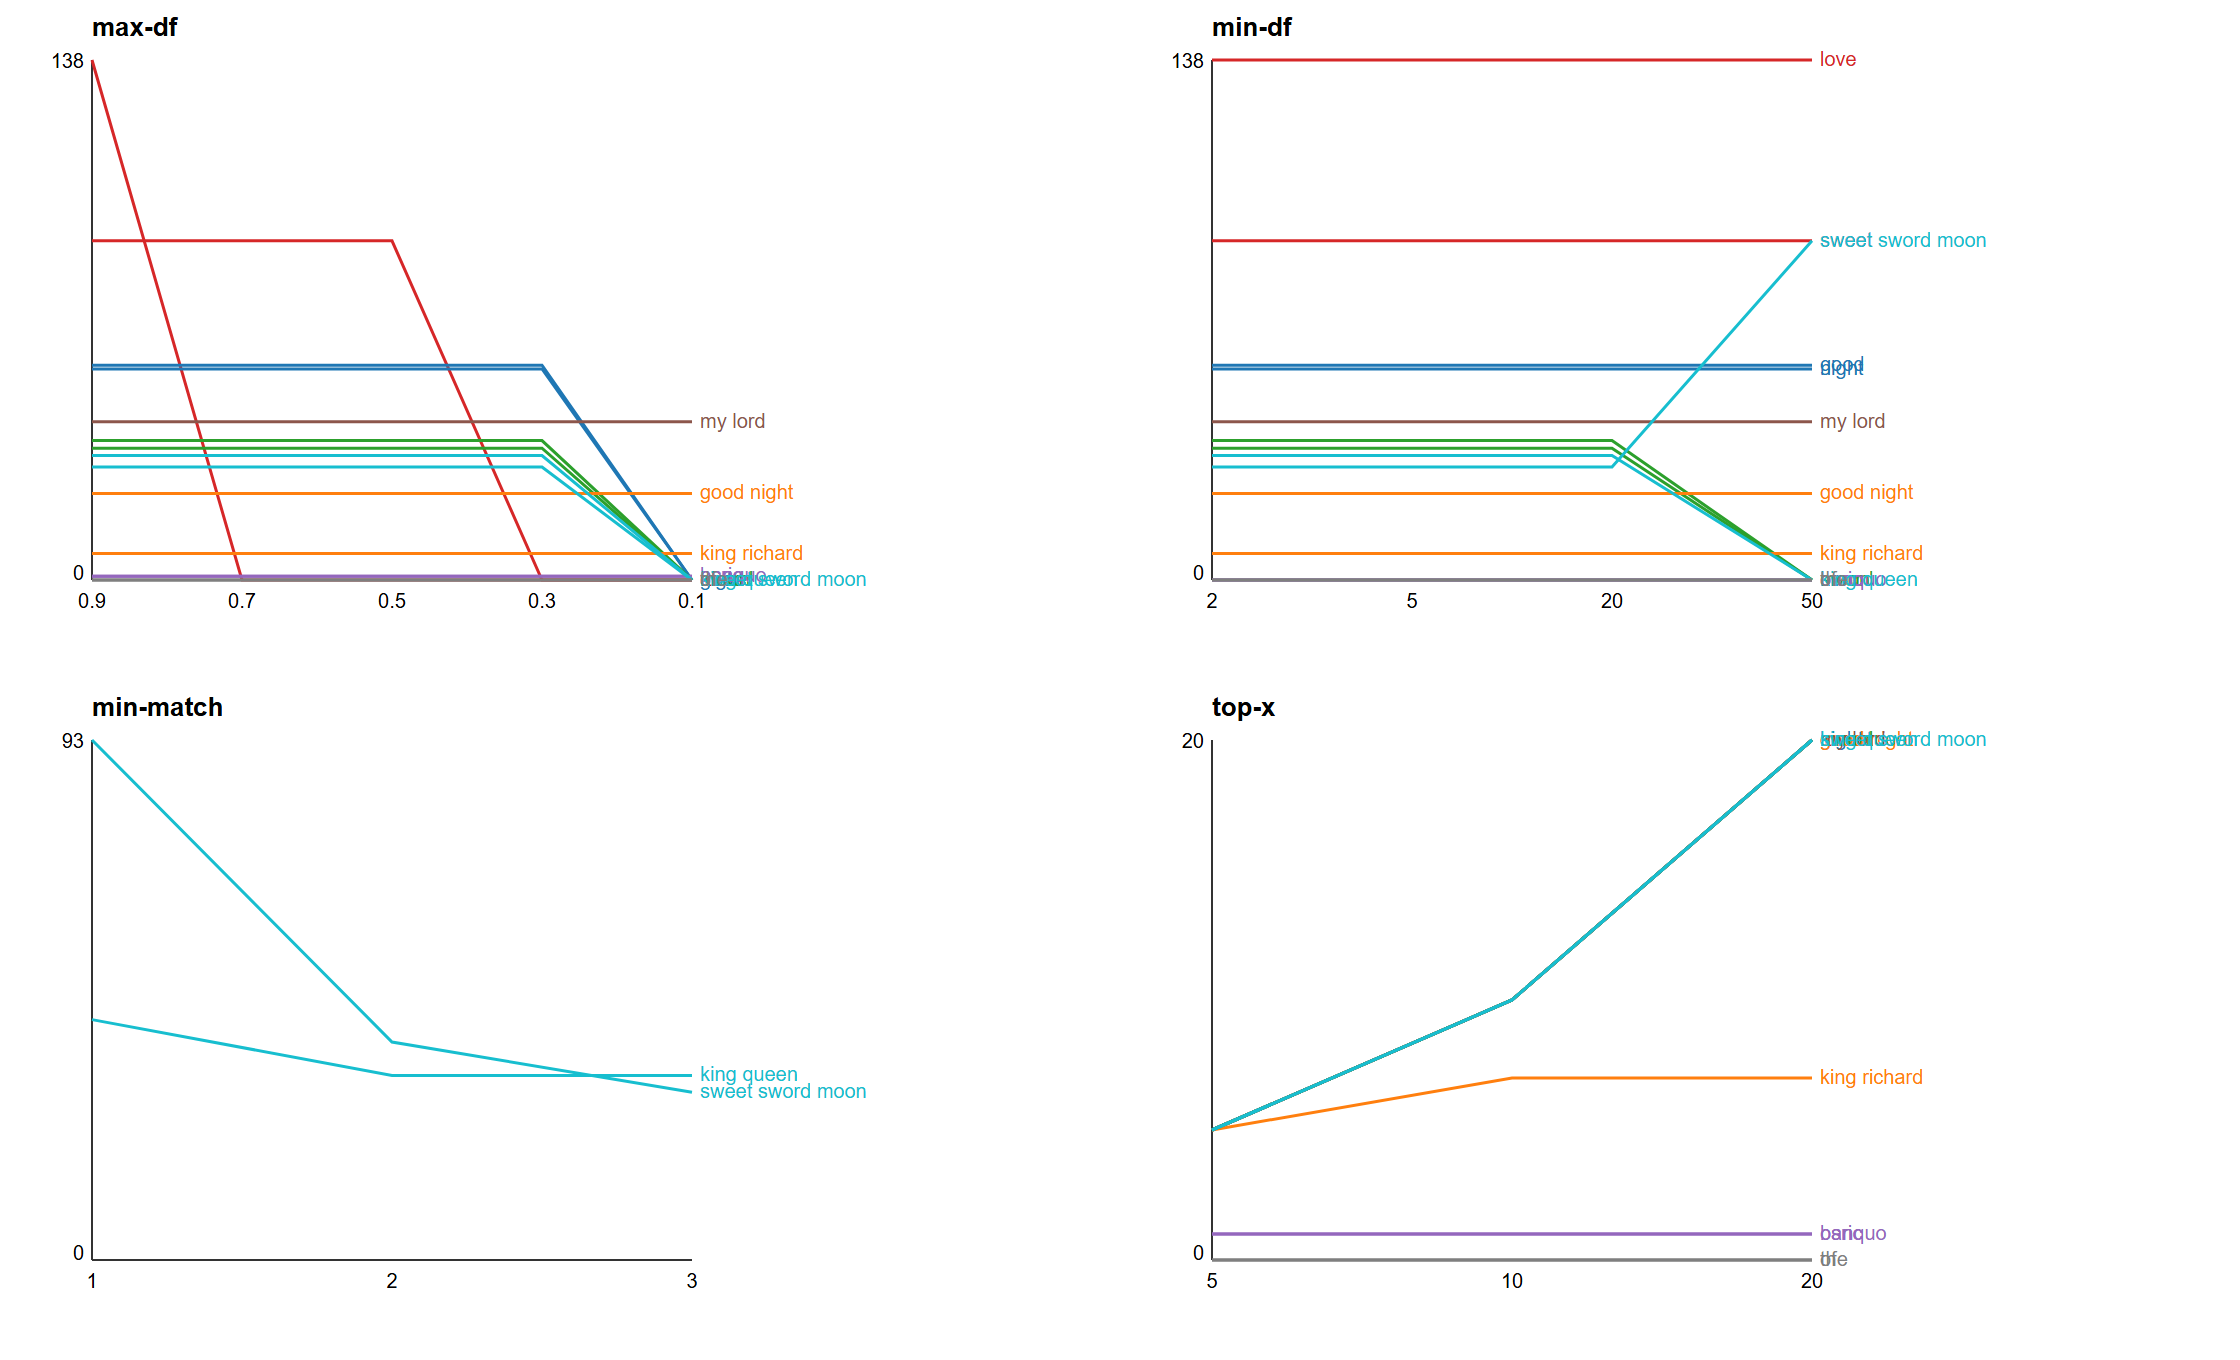
\includegraphics[width=\linewidth]{figures/threshold_matrix.png}
  \caption{阈值矩阵（每个面板一个参数）。\code{--max-df} 与 \code{--min-df} 是词侧截断，\code{--min-match} 是布尔松紧，\code{--top-x} 是结果侧截断；曲线与下表的读数一致。}
  \label{fig:threshold}
\end{figure}

\subsection{\texttt{--max-df}：丢弃“太大众”的词}

\begin{table}[H]
  \centering
  \caption{\texttt{--max-df} 扫描}
  \label{tab:max-df}
  \small
  \begin{tabularx}{\linewidth}{@{}X r r r r r r@{}}
    \toprule
    查询 & 基线 & 0.9 & 0.7 & 0.5 & 0.3 & 0.1 \\
    \midrule
    love（$df\_ratio$ 0.71） & 138 & 138 & 0 & 0 & 0 & 0 \\
    sweet（0.46） & 90 & 90 & 90 & 90 & 0 & 0 \\
    good（0.29） & 57 & 57 & 57 & 57 & 57 & 0 \\
    night（0.29） & 56 & 56 & 56 & 56 & 56 & 0 \\
    sword（0.19） & 37 & 37 & 37 & 37 & 37 & 0 \\
    moon（0.18） & 35 & 35 & 35 & 35 & 35 & 0 \\
    banquo / osric（$df=1$） & 1 & 1 & 1 & 1 & 1 & 1 \\
    king queen & 33 & 33 & 33 & 33 & 33 & 0 \\
    sweet sword moon & 30 & 30 & 30 & 30 & 30 & 0 \\
    短语查询 & 7/23/42 & 7/23/42 & 7/23/42 & 7/23/42 & 7/23/42 & 7/23/42 \\
    the / of & 0 & 0 & 0 & 0 & 0 & 0 \\
    \bottomrule
  \end{tabularx}
\end{table}

\subsection{\texttt{--min-df}：丢弃太罕见的词}

\begin{table}[H]
  \centering
  \caption{\texttt{--min-df} 扫描（最后一行为 \texttt{--min-df 50} 时仅剩 \code{sweet}，Jaccard 0.33）}
  \label{tab:min-df}
  \small
  \begin{tabularx}{\linewidth}{@{}X r r r r r@{}}
    \toprule
    查询 & 基线 & 2 & 5 & 20 & 50 \\
    \midrule
    banquo / osric（$df=1$） & 1 & 0 & 0 & 0 & 0 \\
    sword（$df=37$） & 37 & 37 & 37 & 37 & 0 \\
    moon（$df=35$） & 35 & 35 & 35 & 35 & 0 \\
    king queen & 33 & 33 & 33 & 33 & 0 \\
    sweet sword moon & 30 & 30 & 30 & 30 & 90 \\
    \bottomrule
  \end{tabularx}
\end{table}

\subsection{\texttt{--min-match}：布尔语义松紧}

\begin{table}[H]
  \centering
  \caption{\texttt{--min-match} 扫描（括号内为 Jaccard；$k$ 超过词数时钳制）}
  \label{tab:min-match}
  \small
  \begin{tabularx}{\linewidth}{@{}X r r r r@{}}
    \toprule
    查询 & 基线（AND） & $k=1$ & $k=2$ & $k=3$ \\
    \midrule
    king queen & 33 & 43（0.77） & 33 & 33 \\
    sweet sword moon & 30 & 93（0.32） & 39（0.77） & 30 \\
    \bottomrule
  \end{tabularx}
\end{table}

\subsection{\texttt{--top-x}：结果截断}

\begin{table}[H]
  \centering
  \caption{\texttt{--top-x} 扫描（括号内为 Jaccard）}
  \label{tab:top-x}
  \small
  \begin{tabularx}{\linewidth}{@{}X r r r r@{}}
    \toprule
    查询 & 基线 & 5 & 10 & 20 \\
    \midrule
    love & 138 & 5（0.04） & 10（0.07） & 20（0.14） \\
    good night & 23 & 5（0.22） & 10（0.43） & 20（0.87） \\
    king richard & 7 & 5（0.71） & 7（1.00） & 7（1.00） \\
    banquo / osric & 1 & 1（1.00） & 1（1.00） & 1（1.00） \\
    \bottomrule
  \end{tabularx}
\end{table}

\subsection{关键结论}

\begin{enumerate}
  \item \textbf{\texttt{--max-df} 会直接消除高频词的查询结果}。单词查询一旦词被丢弃，结果从上百篇直接归零；\code{love} 在 0.7 档（$df\_ratio$ 0.71）就被丢弃，\code{sweet} 在 0.3 档被丢弃，说明阈值必须按查询意图设定，不能一律取小。
  \item \textbf{\texttt{--min-df} 与多词 AND 组合会产生反直觉的“丢词即放宽”}。\code{sweet sword moon} 在 \code{--min-df 50} 下丢弃了 \code{sword} 和 \code{moon}，只剩 \code{sweet}，结果从 30 篇增加到 90 篇，Jaccard 仅 0.33。这是“阈值作用于词、而不是作用于结果”的直接后果。
  \item \textbf{\texttt{--min-match} 是布尔语义的松紧旋钮}。$k=1$ 即 OR，结果集显著扩大；$k$ 超过可检索词数时会被钳制，不会返回空集。
  \item \textbf{\texttt{--top-x} 是纯截断}，Jaccard 随 $x$ 单调回升；对结果少的查询（$\le x$）没有影响。
  \item \textbf{短语查询不受 \texttt{--max-df/--min-df} 影响}，Jaccard 恒为 1.00。这是设计行为：短语必须整段匹配，丢弃任何一个词都会改变语义。
  \item \textbf{停用词查询恒为空}，与阈值无关；这是过滤索引的预期行为，输出 note 解释原因。
\end{enumerate}

\section{测试发现并修复的问题}

开发过程中，测试与对拍抓出了十三个真实问题（表~\ref{tab:bugs}）。它们比“全部通过”本身更能说明测试的有效性。

{\footnotesize
\begin{longtable}{@{}r >{\raggedright\arraybackslash}p{0.20\linewidth}
                    >{\raggedright\arraybackslash}p{0.33\linewidth}
                    >{\raggedright\arraybackslash}p{0.33\linewidth}@{}}
  \caption{测试与对拍发现的问题}\label{tab:bugs} \\
  \toprule
  \# & 现象 & 原因 & 处理 \\
  \midrule
  \endfirsthead
  \toprule
  \# & 现象 & 原因 & 处理 \\
  \midrule
  \endhead
  \bottomrule
  \endlastfoot
  1 & 对拍脚本比 C++ 少算 4,340 个 token & 只按行首判断标记行，把 \code{[To HELENA]} 之类台词误判为标题行 & 改为行首与行尾同时匹配，并写入文本层规范 \\
  2 & 正文混入 \code{aside}、\code{sings} 和人名 & 610 处方括号舞台提示被当作正文 & 提取阶段把行首 \code{[...]} 重定位为 \code{(...)} 舞台行；净减 849 token，与片段统计吻合 \\
  3 & 过滤版词频的 \code{tf_share} 分母错误 & C++ 曾把过滤前 token 总数记入 \code{tokens} & 只累计通过过滤器的 token；\code{stopwordTokens} 单独累计；两版 CSV 恢复逐字节一致 \\
  4 & 41 个词形被过度词干化（如 \code{agreem}） & 误以为后缀条件失败后应继续尝试更短后缀 & 改为“首个匹配说了算、条件失败即停”，与 canonical C 一致 \\
  5 & 伸展树插入后段错误 & 插入分支保留了 \code{Node*&} 子指针引用，splay 旋转重接线后引用失效 & 先把新节点指针复制到局部变量，再 splay \\
  6 & 索引加载误报 “index file is truncated” & \code{Reader} 构造时传入了临时 vector；整句结束后 vector 销毁，Reader 持有的引用悬垂 & 先把文件内容存入具名变量，再构造 Reader \\
  7 & v2 压缩索引的 posting offset 全部偏移 & 计算压缩偏移时漏加了 term 表自身大小 & 复用与 v1 相同的 \code{computeTermOffsets()}，v2 只替换 postings 块内容 \\
  8 & 块式构建在真实语料上报 “run 文件截断” & Windows 上 run 文件用文本模式读取，CRLF 被翻译进二进制流 & 显式 \code{std::ios::binary}；golden4 小样本碰巧没有 \code{0x0D0A} 字节对，掩盖了问题 \\
  9 & 字典条目的 \code{term} 字段为空 & 插入时只填了键，没有同步 \code{term} 字段 & 插入后手动设置 \code{entry.term}；随机对拍当场抓住 \\
  10 & B+Tree 的 I2 区间校验误报 & 分隔键是真实键的副本，右子树最左键等于左分隔键 & I2 改为左闭区间 \code{[key[i-1], key[i])} \\
  11 & 变长键下 B+Tree 的 50\% 填充不变量被违反（524 B 小于 528 B 页） & 按条数对半分裂在键长偏斜时不保证字节下界 & 改为“合法窗口内取字节中点”分裂，I3 用可证下界 \code{pageSize/2 - maxEntry} \\
  12 & 磁盘词典查询头部显示 “1 terms” & lazy 路径只把被查询词挂到内存索引，\code{terms.size()} 为 1 & 头部改用 sidecar 的 \code{keyCount()}；文本/JSON 与全量路径逐字节一致 \\
  13 & 30M/50M 键的 B+Tree bulk-load 报 I2 违反 & 内层最右节点借用相邻子节点时，插入了被移动子树的第一个键作为分隔键，而不是原 \code{last} 的首键；该分隔键等于子树最小值，路由会把子树键送到右兄弟 & 插入 \code{last} 原来的首键作为边界；50M 键实测通过（树高 4、4 页读） \\
\end{longtable}
}

另外，讲义四文档的 \code{a} 词项差异（3.3 节）说明：黄金样例本身也需要复核，不能盲目相信参考材料中的二手表格。

\section{小结}

第 3 章的验证链条可以概括为：

\begin{lstlisting}[language=,basicstyle=\ttfamily\small]
单元测试（模块行为）
   + 黄金样例（已知输入/输出）
   + 独立 Python 对拍（同一规格的第二实现）
   + 不变量校验（结构自洽）
   + 全量 brute-force（从原始文本重建期望）
   = 对索引正确性的高置信度
\end{lstlisting}

阈值实验则回答了任务 (4)：四个参数分别从“词侧”和“结果侧”改变结果集，且不同查询类型（单词、短语、布尔、停用词）对阈值的反应不同。具体分析见第 4 章。Bonus 的验证链在同一套方法上继续扩展：熵规则与人工表对照、RFC 第二语料端到端对拍、v2 压缩、块式构建、B+Tree 三条独立对拍，结果见 3.4 到 3.6 节。
